% ------------------------------------------------------------------------------
% Este fichero es parte de la plantilla LaTeX para la realización de Proyectos
% Final de Grado, protegido bajo los términos de la licencia GFDL.
% Para más información, la licencia completa viene incluida en el
% fichero fdl-1.3.tex

% Copyright (C) 2012 SPI-FM. Universidad de Cádiz
% ------------------------------------------------------------------------------

En este capítulo se documentan los diferentes tipos de pruebas que se han
llevado a cabo, ya sean de carácter manual o automatizadas mediante software
específico de pruebas.

\section{Pruebas unitarias y de integración}

Para el desarrollo de las pruebas unitarias y de integración de los distintos
artefactos software desarrollados, se han realizado una serie de pruebas
automatizadas mediante el framework de Python para el desarrollo de pruebas
PyUnit, el cual está basado en el framework de pruebas JUnit de Java.

Mediante las pruebas automáticas desarrolladas, se ha probado que tanto los
modelos y métodos de que disponen los mismos realizan las funciones para las que
han sido desarrollados correctamente. Además, también se ha probado la
integración entre los mismos, así como las distintas funciones auxiliares
desarrolladas, donde se combinan el uso de los distintos modelos, así como sus
métodos.

Para lanzar La ejecución de las distintas pruebas automáticas diseñadas, se hará
de la siguiente forma, desde una terminal de escritorio en el directorio donde
se encuentre el fichero manage.py de nuestro proyecto Django:

\begin{lstlisting}[frame=L, language=bash, basicstyle=\footnotesize]
$> python manage.py test easydata
\end{lstlisting}

Esto muestra un informe de los distintos tests ejecutados, así como los posibles
errores que hayan podido surgir en los mismos si alguna de las funciones no se
llevado a cabo tal y como se esperaba. El resultado de la validación debe de ser
similar al que puede apreciarse en la siguiente figura (\ref{fig:pyunit}).

\begin{figure}[H]
    \begin{center}
        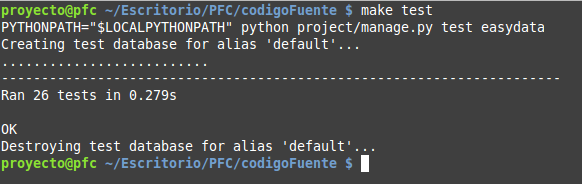
\includegraphics[width=1\textwidth]{pruebas/pyunit.png}
    \end{center}
    \caption{Resultado de validación PyUnit}
    \label{fig:pyunit}
\end{figure}

Adicionalmente, al tratarse de una aplicación la cual se instalará en proyectos
Django ya existentes, se ha probado su integración con aplicaciones disponibles
en el \textit{Python Package Index} desarrolladas por otros autores. Más
concretamente, para el desarrollo de las pruebas que se muestran a continuación,
se ha utilizado la aplicación django-blog-zinnia, que como su nombre indica, se
trata de un blog escrito en Python para Django.

%Las pruebas unitarias tienen por objetivo localizar errores en cada nuevo artefacto software desarrollado, antes que se produzca la integración con el resto de artefactos del sistema. 

%Este tipo de pruebas tienen por objetivo localizar errores en módulos o subsistemas completos, analizando la interacción entre varios artefactos software.


\section{Pruebas de sistema}

En este apartado se describen las pruebas de sistema de modo que se asegure que
el sistema cumple con todos los requisitos establecidos al comienzo del
proyecto, bajo un entorno específico para pruebas.

Para ello se han realizado pruebas manuales, donde se ha comprobado que se
cumplen los requisitos funcionales especificados inicialmente, accediendo a los
distintos apartados de:
\begin{itemize}
    \item \textbf{Captación de modelos y fields del proyecto Django:} se ha
        probado que la carga de modelos y fields del proyecto funciona
        correctamente, así como la actualización de los datos antes posibles
        cambios en los modelos.
    \item \textbf{Carga de nuevos namespaces:} se ha probado que la carga de
        nuevos namespaces u ontologías funciona correctamente, además de la
        actualización de la especificación de los mismos ante posibles cambios.
        Para ello se ha probado con multitud de namespaces diferentes
        suministrados por distintas organizaciones.
    \item \textbf{Configuración de la visibilidad de los modelos y fields:} se
        ha probado que tanto el proceso de configuración de la visibilidad
        funcione correctamente, como que a la hora de publicar los datos,
        aquellos marcados como no visibles no se publiquen a los usuarios
        utilizando las diferentes herramientas de publicación de datos.
    \item \textbf{Mapeo de modelos y fields:} se ha probado que el mapeo de los
        datos funciona correctamente utilizando varios namespaces de forma
        individual o simultánea para un mismo modelo. Posteriormente, se ha
        comprobado que los datos se publican haciendo uso de las etiquetas
        especificadas en este apartado de configuración.
    \item \textbf{Publicación de datos en RDF, RDFa y Microdata:} Una vez
        realizada tanto la carga de modelos y fields, como la configuración de
        los mismos comentada anteriormente, se ha probado que estos se publican
        correctamente según los criterios especificados.
    \item \textbf{Herramienta de generación de D2Rq:} se ha probado que una vez
        realizada la configuración de los modelos y fields, se genera el fichero
        con la configuración para el software D2Rq y este funciona correctamente
        con la aplicación, probando consultas SPARQL y comprobando que los
        resultados sean satisfactorios.
    \item \textbf{Generación de diagrama con configuración:} una vez realizada
        la configuración de los modelos y los fields, se ha probado que la
        generación del diagrama con la configuración mediante Graphviz, se
        corresponde con la configuración realizada.
\end{itemize}

Además de la comprobación de que se han satisfacido cada uno de los requisitos
funcionales descritos en el apartado de análisis del proyecto, se han realizado
pruebas de validación, de los datos exportados.

A continuación se muestra un resumen de las pruebas de validación realizadas
sobre los datos publicados por la aplicación EasyData/Django.

\subsection{Pruebas no funcionales} 

\subsubsection{Pruebas de validación de RDF}

La validación del código RDF generado por la aplicación EasyData/Django, se ha
hecho uso del validador suministrado por el W3C
(\url{http://www.w3.org/RDF/Validator/}). Para la realización de la prueba, se
suministró al validador del W3C diferentes salidas proporcionadas por la
aplicación EasyData/Django, comprobando en cada caso que el resultado de la
validación fuese satisfactorio. De esta forma, obtenemos la seguridad de que los
datos RDF publicados, están perfectamente generados y cumple estrictamente los
estándares impuestos por el W3C.

A continuación, se muestra un ejemplo de una salida generada por la aplicación
EasyData/Django en formato RDF/XML, para una entrada de blog de la aplicación
anteriormente comentada, donde se pueden apreciar las marcas que se han añadido
en función del mapeo realizado.

\begin{lstlisting}[frame=L, language=bash, basicstyle=\footnotesize, breaklines=true, numbers=left]
<?xml version="1.0" encoding="UTF-8"?>
<rdf:RDF
   xmlns:foaf="http://xmlns.com/foaf/0.1/"
   xmlns:rdf="http://www.w3.org/1999/02/22-rdf-syntax-ns#"
   xmlns:schema="http://schema.org/"
>
  <rdf:Description rdf:about="http://pfc-llerena.rhcloud.com/easydata/publish/instance/zinnia/BlogPosting-Entry/2.xml">
    <schema:sameAs>Esta es la segunda entrada del blog de zinnia.Ten mucha suerte en tu Proyecto Fin de Carrera.</schema:sameAs>
    <schema:dateModified rdf:datatype="http://www.w3.org/2001/XMLSchema#dateTime">2013-12-01T11:36:17.142964</schema:dateModified>
    <foaf:skypeID rdf:datatype="http://www.w3.org/2001/XMLSchema#integer">2</foaf:skypeID>
    <schema:text>&lt;p&gt;Esta es la segunda entrada del blog de zinnia.&lt;/p&gt;&lt;p&gt;Ten mucha suerte en tu Proyecto Fin de Carrera.&lt;/p&gt;</schema:text>
    <schema:description rdf:datatype="http://www.w3.org/2001/XMLSchema#boolean">false</schema:description>
    <schema:keywords></schema:keywords>
    <foaf:myersBriggs>None</foaf:myersBriggs>
    <rdf:type rdf:resource="http://schema.org/BlogPosting"/>
    <schema:dateCreated rdf:datatype="http://www.w3.org/2001/XMLSchema#dateTime">2013-12-01T11:35:33</schema:dateCreated>
    <schema:datePublished rdf:datatype="http://www.w3.org/2001/XMLSchema#dateTime">2013-12-01T11:36:11</schema:datePublished>
    <schema:headline>Segunda entrada</schema:headline>
    <foaf:page>entry_detail.html</foaf:page>
    <schema:sameAs>segunda-entrada</schema:sameAs>
    <schema:award rdf:datatype="http://www.w3.org/2001/XMLSchema#integer">0</schema:award>
    <schema:about rdf:resource="http://pfc-llerena.rhcloud.com/easydata/publish/instance/zinnia/BlogPosting-Entry/1.xml"/>
  </rdf:Description>
</rdf:RDF>
\end{lstlisting}

En la figura \ref{fig:rdftest} se puede apreciar una captura de pantalla con el
resultado de la validación devuelto por el validador del W3C, donde se puede
ver que el código RDF cumple con los estándares impuestos por el W3C.

\newpage

\begin{figure}[H]
    \begin{center}
        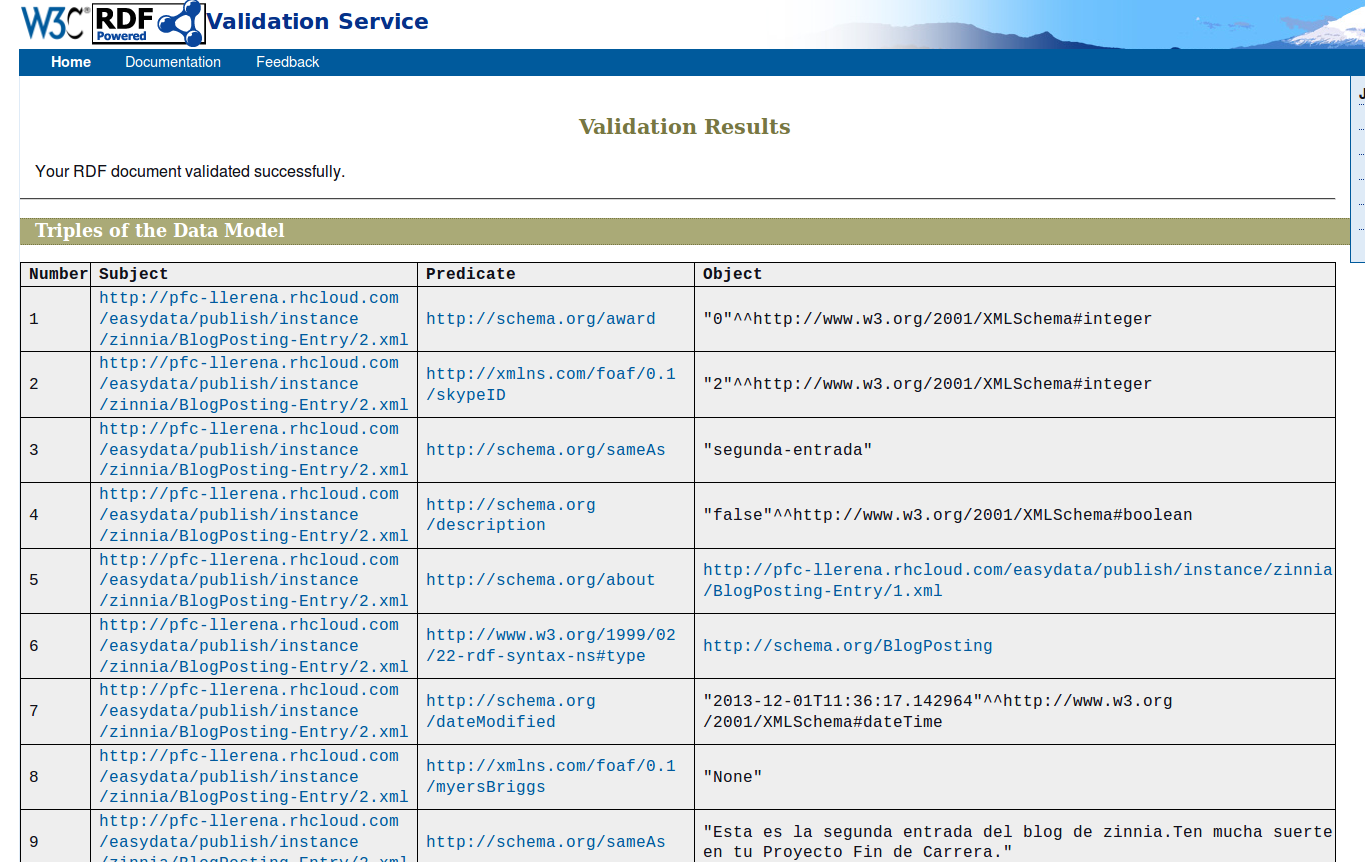
\includegraphics[width=1\textwidth]{pruebas/rdftest.png}
    \end{center}
    \caption{Resultado de validación RDF}
    \label{fig:rdftest}
\end{figure}


\subsubsection{Pruebas de validación de RDFa}

Al igual que para el caso de RDF, también se ha realizado una validación del
código RDFa generado por la aplicación EasyData/Django, haciendo uso de igual
forma del validador suministrado por el W3C
(\url{http://www.w3.org/2012/pyRdfa/Validator.html}). Para la realización de las
pruebas, se suministró al validador del W3C diferentes salidas proporcionadas
por la aplicación EasyData/Django, comprobando en cada caso que el resultado de
la validación fuese satisfactorio. Así de esta forma, nos aseguramos también que
el código RDFa generado por la aplicación, están perfectamente generado y cumple
de igual forma estrictamente los estándares impuestos por el W3C.

A continuación, se muestra un ejemplo de una salida generada por la aplicación
EasyData/Django en formato RDFa, para una entrada de blog de la aplicación
anteriormente comentada, donde se pueden apreciar las marcas que se han añadido
en función del mapeo realizado al lenguaje HTML utilizando la notación RDFa.

\begin{lstlisting}[frame=L, language=HTML, basicstyle=\footnotesize, breaklines=true, numbers=left]
<div about="http://pfc-llerena.rhcloud.com/easydata/publish/instance/zinnia/BlogPosting-Entry/2.xml" typeof="schema:BlogPosting" prefix="schema: http://schema.org/ foaf: http://xmlns.com/foaf/0.1/">
    <div content="2" property="foaf:skypeID"></div>
    <div content="Segunda entrada" property="schema:headline"></div>
    <div content="segunda-entrada" property="schema:sameAs"></div>
    <div content="2013-12-01 11:36:11" property="schema:datePublished"></div>
    <div content="None" property="foaf:myersBriggs"></div>
    <div content="2013-12-01 11:35:33" property="schema:dateCreated"></div>
    <div content="2013-12-01 11:36:17.142964" property="schema:dateModified"></div>
    <div content="&lt;p&gt;Esta es la segunda entrada del blog de zinnia.&lt;/p&gt;&lt;p&gt;Ten mucha suerte en tu Proyecto Fin de Carrera.&lt;/p&gt;" property="schema:text"></div>
    <div content="0" property="schema:award"></div>
    <div content="Esta es la segunda entrada del blog de zinnia.Ten mucha suerte en tu Proyecto Fin de Carrera." property="schema:sameAs"></div>
    <div content="" property="schema:keywords"></div>
    <div content="False" property="schema:description"></div>
    <div content="entry_detail.html" property="foaf:page"></div>
    <link resource="http://pfc-llerena.rhcloud.com/easydata/publish/instance/zinnia/BlogPosting-Entry/1.xml" rel="schema:about">
</div>

<div about="http://pfc-llerena.rhcloud.com/easydata/publish/instance/zinnia/BlogPosting-Entry/1.xml" typeof="schema:BlogPosting" prefix="schema: http://schema.org/ foaf: http://xmlns.com/foaf/0.1/">
    <div content="1" property="foaf:skypeID"></div>
    <div content="Saludo inicial" property="schema:headline"></div>
    <div content="saludo-inicial" property="schema:sameAs"></div>
    <div content="2013-12-01 11:01:17" property="schema:datePublished"></div>
    <div content="None" property="foaf:myersBriggs"></div>
    <div content="2013-12-01 11:00:40" property="schema:dateCreated"></div>
    <div content="2013-12-01 11:01:36.367237" property="schema:dateModified"></div>
    <div content="&lt;p&gt;Esto es una entrada de prueba para el blog de zinnia para probar junto con EasyData.&lt;/p&gt;" property="schema:text"></div>
    <div content="0" property="schema:award"></div>
    <div content="Esto es una entrada de prueba para el blog de zinnia para probar junto con EasyData." property="schema:sameAs"></div>
    <div content="easydata" property="schema:keywords"></div>
    <div content="False" property="schema:description"></div>
    <div content="entry_detail.html" property="foaf:page"></div>
    <link resource="http://pfc-llerena.rhcloud.com/easydata/publish/instance/zinnia/BlogPosting-Entry/2.xml" rel="schema:about">
</div>
\end{lstlisting}

En la figura \ref{fig:rdfatest} se puede apreciar una captura de pantalla con el
resultado de la validación producido por el validador del W3C, donde se puede
ver que el código RDFa cumple con los estándares impuestos por el W3C.

\newpage

\begin{figure}[H]
    \begin{center}
        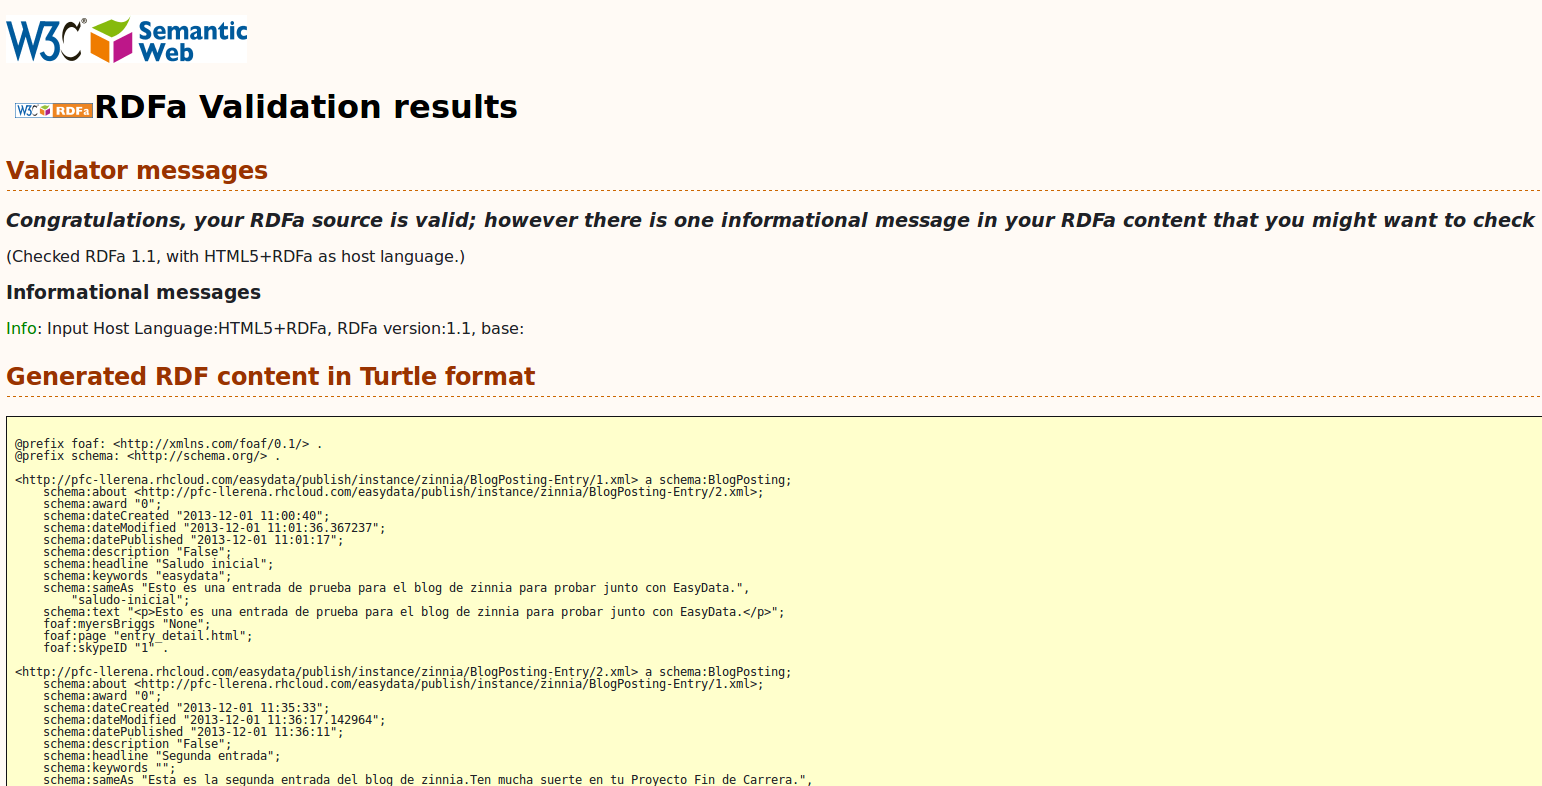
\includegraphics[width=1\textwidth]{pruebas/rdfatest.png}
    \end{center}
    \caption{Resultado de validación RDFa}
    \label{fig:rdfatest}
\end{figure}


\subsubsection{Pruebas de validación de Microdata}

Por último, al igual que en los casos anteriores, también se ha realizado una
validación del código Microdata generado por la aplicación EasyData/Django,
haciendo uso de una herramienta suministrada por Google
(\url{http://www.google.com/webmasters/tools/richsnippets}), la cual busca
metadatos en una determinada URI que se le suministre. Para la realización de la
prueba, se suministró a la herramienta de Google diferentes salidas
proporcionadas por la aplicación EasyData/Django, comprobando en cada caso que
los datos captados por la herramienta fuesen los correctos. Así de esta forma,
nos aseguramos también que el código Microdata generado por la aplicación, está
correctamente construido.

A continuación, se muestra un ejemplo de una salida generada por la aplicación
EasyData/Django en formato Microdata, para una entrada de blog de la aplicación
anteriormente comentada, donde se pueden apreciar las marcas que se han añadido
en función del mapeo realizado al lenguaje HTML utilizando la notación Microdata.

\begin{lstlisting}[frame=L, language=HTML, basicstyle=\footnotesize, breaklines=true, numbers=left]
<div itemid="http://pfc-llerena.rhcloud.com/easydata/publish/instance/zinnia/BlogPosting-Entry/2.xml" itemtype="http://schema.org/BlogPosting" itemscope >
    <span itemprop="http://xmlns.com/foaf/0.1/skypeID">2</span>
    <span itemprop="http://schema.org/headline">Segunda entrada</span>
    <span itemprop="http://schema.org/sameAs">segunda-entrada</span>
    <span itemprop="http://schema.org/datePublished">2013-12-01 11:36:11</span>
    <span itemprop="http://xmlns.com/foaf/0.1/myersBriggs">None</span>
    <span itemprop="http://schema.org/dateCreated">2013-12-01 11:35:33</span>
    <span itemprop="http://schema.org/dateModified">2013-12-01 11:36:17.142964</span>
    <span itemprop="http://schema.org/text"><p>Esta es la segunda entrada del blog de zinnia.</p><p>Ten mucha suerte en tu Proyecto Fin de Carrera.</p></span>
    <span itemprop="http://schema.org/award">0</span>
    <span itemprop="http://schema.org/sameAs">Esta es la segunda entrada del blog de zinnia.Ten mucha suerte en tu Proyecto Fin de Carrera.</span>
    <span itemprop="http://schema.org/keywords"></span>
    <span itemprop="http://schema.org/description">False</span>
    <span itemprop="http://xmlns.com/foaf/0.1/page">entry_detail.html</span>
    <link href="http://pfc-llerena.rhcloud.com/easydata/publish/instance/zinnia/BlogPosting-Entry/1.xml" itemprop="http://schema.org/about">
</div>

<div itemid="http://pfc-llerena.rhcloud.com/easydata/publish/instance/zinnia/BlogPosting-Entry/1.xml" itemtype="http://schema.org/BlogPosting" itemscope >
    <span itemprop="http://xmlns.com/foaf/0.1/skypeID">1</span>
    <span itemprop="http://schema.org/headline">Saludo inicial</span>
    <span itemprop="http://schema.org/sameAs">saludo-inicial</span>
    <span itemprop="http://schema.org/datePublished">2013-12-01 11:01:17</span>
    <span itemprop="http://xmlns.com/foaf/0.1/myersBriggs">None</span>
    <span itemprop="http://schema.org/dateCreated">2013-12-01 11:00:40</span>
    <span itemprop="http://schema.org/dateModified">2013-12-01 11:01:36.367237</span>
    <span itemprop="http://schema.org/text"><p>Esto es una entrada de prueba para el blog de zinnia para probar junto con EasyData.</p></span>
    <span itemprop="http://schema.org/award">0</span>
    <span itemprop="http://schema.org/sameAs">Esto es una entrada de prueba para el blog de zinnia para probar junto con EasyData.</span>
    <span itemprop="http://schema.org/keywords">easydata</span>
    <span itemprop="http://schema.org/description">False</span>
    <span itemprop="http://xmlns.com/foaf/0.1/page">entry_detail.html</span>
    <link href="http://pfc-llerena.rhcloud.com/easydata/publish/instance/zinnia/BlogPosting-Entry/2.xml" itemprop="http://schema.org/about">
</div>
\end{lstlisting}

En la figura \ref{fig:microdatatest} se puede apreciar una captura de pantalla
con el resultado de la validación producido por el validador de Google, donde se
puede ver que que se extraen correctamente los datos del código Microdata.

\newpage

\begin{figure}[H]
    \begin{center}
        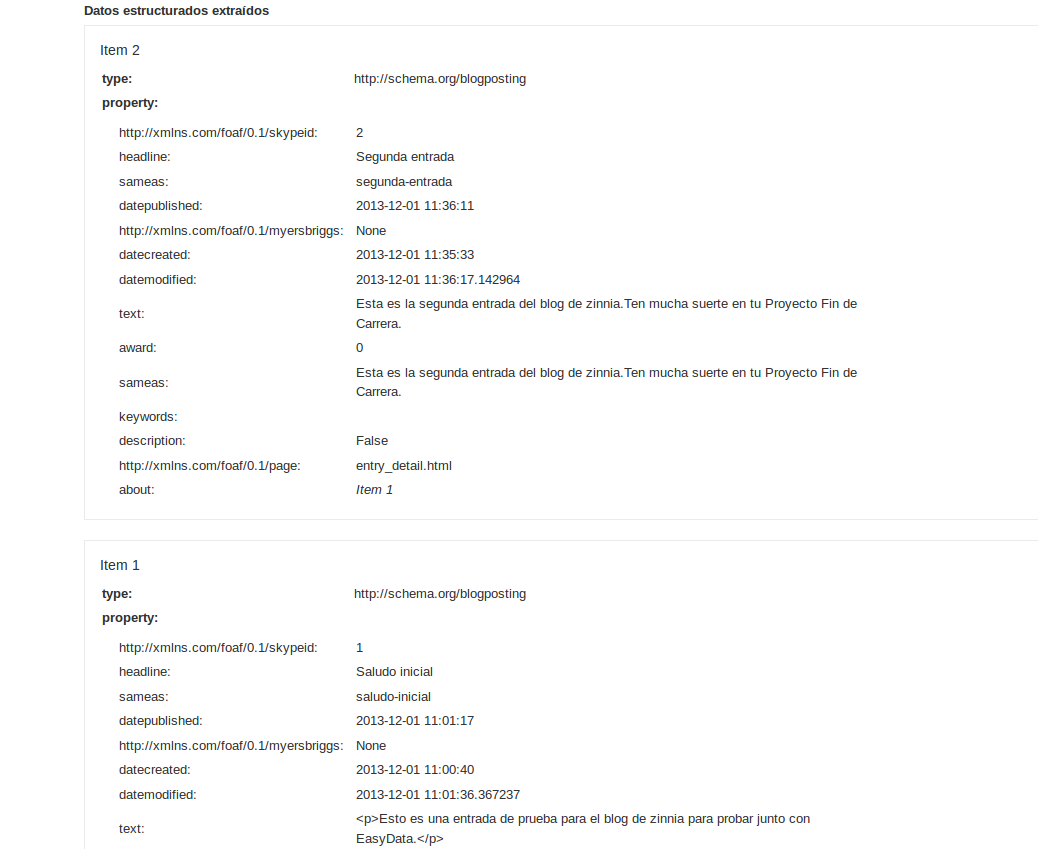
\includegraphics[width=1\textwidth]{pruebas/microdatatest.png}
    \end{center}
    \caption{Resultado de validación Microdata}
    \label{fig:microdatatest}
\end{figure}

\subsubsection{Resto de pruebas no funcionales}

Por otro lado, para llevar a cabo el resto de pruebas no funcionales, se ha
realizado una validación manual, asegurándonos de que se cumplen el resto de
requisitos no funcionales impuestos para la aplicación, como son:
\begin{itemize}
    \item \textbf{Seguridad:} comprobando que las vistas son únicamente
        accesibles para usuarios administradores de Django, y que únicamente se
        publican aquellos datos que el usuario ha marcado como visibles.
    \item \textbf{Portabilidad:} habiéndose usado siempre herramientas
        compatibles con python, o soportadas por múltiples plataformas.
    \item \textbf{Entorno tecnológico:} se ha desarrollado una aplicación
        perfectamente compatible con las versiones iguales o superiores a Django
        1.4.
    \item \textbf{Mantenibilidad:} se trata de una aplicación desarrollada como
        un paquete python, el cual cumple con las reglas impuestas por el PEP8
        para la escritura de código y habiéndose realizado una evaluación de la
        calidad del código fuente con la herramienta PyLint.
\end{itemize}

% Estas pruebas pretenden comprobar el funcionamiento del sistema, con respecto a los requisitos no funcionales definidos en la etapa de análisis: rendimiento, accesibilidad, etc. 

% \section{Pruebas de aceptación}
% El objetivo de estas pruebas es demostrar que el producto está listo para el paso a producción. Suelen ser las mismas pruebas que se realizaron anteriormente pero en el entorno de producción. En estas pruebas, es importante la participación del cliente final.
